\begin{savequote}[75mm]
I rarely find it useful to distinguish between theory and practice; their interplay is already profound and will only increase as the systems and problems we consider grow more complex.
\qauthor{Michael I. Jordan}
\end{savequote}

\chapter{A Web Implementation of the Luna Rating System}

\section{Introduction}

The Luna Rating System is designed to be a practical test for machine intelligence. It may offer some utility as a thought experiment, but its primary value can only be realized in practice. In this chapter, I describe the design and launch of the first web-based implementation of LRS. The application is meant to serve as a comprehensive proof-of-concept. For the application to fulfill its purpose, it must first be capable of recruiting and handling hundreds of human players. The design should then persuade players to play several games, so as to refine their Smarts Ratings. Finally, the behavior of players should indicate a collective understanding of the Luna Game, and evidence should suggest their aspirations towards honest play.

The baseline success of the LRS implementation can be easily measured through traffic statistics: how many players play, and how long do they typically stay? Such statistics comprise the first section of results in this chapter. In addition to these standard metrics, the questions and responses traded by the players can be assessed qualitatively. I provide a representative sample of questions and discuss common themes from the full dataset. The final source of results is derived from human players' interactions with simple standardized machine players. I argue that the Guesses that human players make of the machine players should converge over time as a consensus on the semantics of Smarts Ratings is reached. The introduction of machine players also provides a demonstration for AI researchers who wish to introduce their own machines into the system.

\section{Building the Web Interface}

\subsection{Design of the Web Interface}

My implementation of the Luna Rating System is built on the open-source software stack consisting of MongoDB, Express.js, Angular.js, and Node.js, which is collectively referred to as the MEAN stack\cite{meanstack}. The latter three technologies are all written in JavaScript and MongoDB is a NoSQL database. At a very high level, MongoDB stores all player and game data, Angular.js controls and displays the client side, Express.js forms the foundation of the server side, and Node.js runs the code written on top of that foundation. Notable libraries used include Mongoose.js, a Node.js library for interfacing with MongoDB; Passport.js, a Node.js library which provides middleware for user authentication; and Angular-UI, an Angular.js library that simplifies routing, i.e. navigation between different states of the website. To protect user anonymity, usernames are hashed on the client side using MD5. The front end of the website, i.e. the style, formatting, and organization of content, was modified from the ``Material Admin'' LESS/Angular.js template, for which I purchased a single application license\cite{materials}. The site was developed locally and then hosted on EC2 by Amazon Web Services under the domain name ``luna-game.com''.

The skeletal framework of the website was first paper-prototyped and then iterated upon\cite{paperproto}. The centerpiece of the website is the ongoing Luna Games, and a secondary component allows users to review their performance in previous Games. A single Luna Game seamlessly transitions from one phase to the next, while retaining cohesion as a whole Game. All opportunities for latency --- between phases of a Game or between Games ---  are reduced as much as possible to encourage repeated play. To increase the probability that a first-time user explores the website beyond the landing page, the website has an option to play as a ``guest.'' The only functional difference between a user that signs up and a guest is that signed up users may log out and log back in, while a guest account expires once the 60-day token is removed from the browser or the user signs out. User experience was further considered in the context of the results presented in Chapter 3 of this thesis, which demonstrates that all players must have a clear understanding of their goals during a Luna Game. While users should be able to start playing Luna Games as quickly as possible, they should first be fully aware of the Game's structure and their goals.

Weighing these considerations, the core features of the website are divided into 10 primary states and 4 secondary states. The secondary states include static pages --- the contact page and two extended information pages --- and one profile page that allows a user to review statistics related to her historical performance. The primary states are presented in Figure \ref{statediagram}. They include four states corresponding to the phases of a Luna game, one home state, which contains games as nested states, a landing page, a guest state, a sign up state, a login state, and an information state. Note that first-time users must provide consent and review information about the structure of Luna Games before they are able to play. The eager first-time user is able to reach a new game with only three clicks from the home page, and a returning user can reach games with two clicks and a form submission. This simple state architecture ensures that users are informed and playing as soon as possible. Screen shots of a typical user experience are depicted in Figure \ref{screenshotpic}.

\begin{figure}
\begin{scriptsize}
\begin{center}
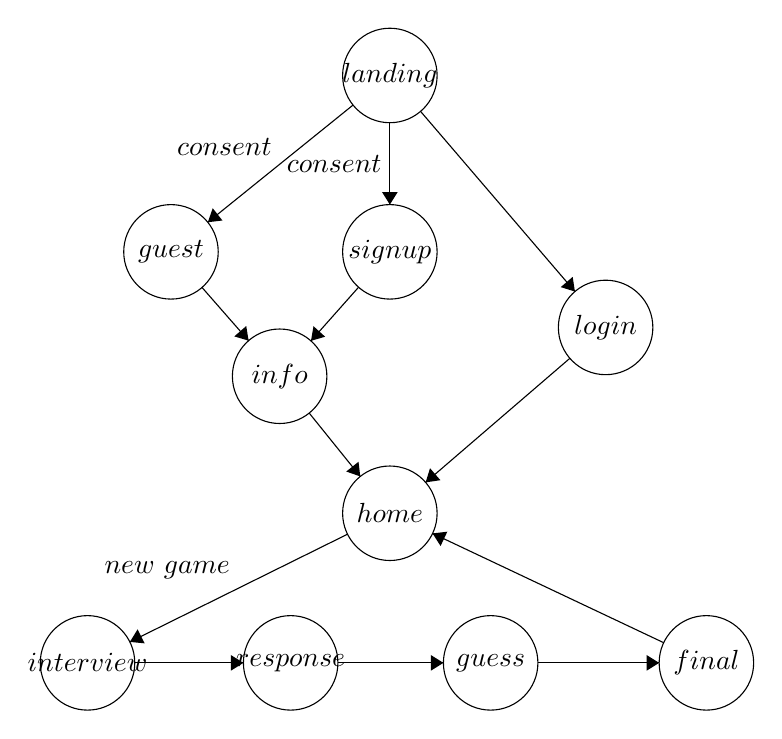
\begin{tikzpicture}[scale=0.2]
\tikzstyle{every node}+=[inner sep=0pt]
\draw [black] (38.9,-3.4) circle (3);
\draw (38.9,-3.4) node {$landing$};
\draw [black] (25,-14.6) circle (3);
\draw (25,-14.6) node {$guest$};
\draw [black] (38.9,-14.6) circle (3);
\draw (38.9,-14.6) node {$signup$};
\draw [black] (52.6,-19.4) circle (3);
\draw (52.6,-19.4) node {$login$};
\draw [black] (38.9,-31.2) circle (3);
\draw (38.9,-31.2) node {$home$};
\draw [black] (19.7,-40.7) circle (3);
\draw (19.7,-40.7) node {$interview$};
\draw [black] (32.6,-40.7) circle (3);
\draw (32.6,-40.7) node {$response$};
\draw [black] (45.3,-40.7) circle (3);
\draw (45.3,-40.7) node {$guess$};
\draw [black] (59,-40.7) circle (3);
\draw (59,-40.7) node {$final$};
\draw [black] (31.9,-22.5) circle (3);
\draw (31.9,-22.5) node {$info$};
\draw [black] (38.9,-6.4) -- (38.9,-11.6);
\fill [black] (38.9,-11.6) -- (39.4,-10.8) -- (38.4,-10.8);
\draw (38.4,-9) node [left] {$consent$};
\draw [black] (36.56,-5.28) -- (27.34,-12.72);
\fill [black] (27.34,-12.72) -- (28.27,-12.61) -- (27.65,-11.83);
\draw (28.39,-8.51) node [above] {$consent$};
\draw [black] (40.85,-5.68) -- (50.65,-17.12);
\fill [black] (50.65,-17.12) -- (50.51,-16.19) -- (49.75,-16.84);
\draw [black] (50.33,-21.36) -- (41.17,-29.24);
\fill [black] (41.17,-29.24) -- (42.11,-29.1) -- (41.45,-28.34);
\draw [black] (36.21,-32.53) -- (22.39,-39.37);
\fill [black] (22.39,-39.37) -- (23.33,-39.46) -- (22.88,-38.57);
\draw (24.76,-35.43) node [above] {$new\mbox{ }game$};
\draw [black] (22.7,-40.7) -- (29.6,-40.7);
\fill [black] (29.6,-40.7) -- (28.8,-40.2) -- (28.8,-41.2);
\draw [black] (35.6,-40.7) -- (42.3,-40.7);
\fill [black] (42.3,-40.7) -- (41.5,-40.2) -- (41.5,-41.2);
\draw [black] (48.3,-40.7) -- (56,-40.7);
\fill [black] (56,-40.7) -- (55.2,-40.2) -- (55.2,-41.2);
\draw [black] (56.29,-39.42) -- (41.61,-32.48);
\fill [black] (41.61,-32.48) -- (42.12,-33.28) -- (42.55,-32.37);
\draw [black] (33.78,-24.84) -- (37.02,-28.86);
\fill [black] (37.02,-28.86) -- (36.91,-27.93) -- (36.13,-28.55);
\draw [black] (26.97,-16.86) -- (29.93,-20.24);
\fill [black] (29.93,-20.24) -- (29.78,-19.31) -- (29.02,-19.97);
\draw [black] (36.91,-16.85) -- (33.89,-20.25);
\fill [black] (33.89,-20.25) -- (34.79,-19.99) -- (34.05,-19.32);
\end{tikzpicture}
\end{center}
\end{scriptsize}
\caption{Schematic diagram depicting the primary states of the Luna Rating System web interface. Nodes represent website states and edges indicate how users typically navigate between states. A first-time user arrives at the \textit{landing} state. Upon providing consent, the user may play as a \textit{guest} or \textit{sign up}, both which lead to the \textit{info} state. The info state explains the Luna Game and then directs users to the \textit{home} state. The user can then create a new Luna Game, launching the \textit{interview} state. As the user progresses through the Luna Game, she transitions from interview to \textit{response}, to \textit{guess}, and to \textit{final}. They then return to the home state to start another game. Returning signed up users may \textit{login} from the landing state to reach the home state.}
\label{statediagram}
\end{figure}

\begin{figure}
\includegraphics[width=0.5\textwidth]{figures/screen1.png}
\includegraphics[width=0.5\textwidth]{figures/screen2.png}
\includegraphics[width=0.5\textwidth]{figures/screen3.png}
\includegraphics[width=0.5\textwidth]{figures/screen4.png}
\includegraphics[width=0.5\textwidth]{figures/screen5.png}
\includegraphics[width=0.5\textwidth]{figures/screen6.png}
\caption{Exemplary screenshots of the Luna website. Clockwise from top left: the landing page, the information page for first-time users, interview phase, response phase, guess phase, and final phase.}
\label{screenshotpic}
\end{figure}
\subsection{An API for Machine Players}

To allow AI researchers to enter machines as players on the Luna Rating System website, I implemented a RESTful API. Machine players must first register separately from human players to receive an API token. This process is currently done by hand, since the system is not yet protected against malicious machine players (e.g. there is no limit on the number of API calls that one player may make). With an API token obtained, the experience of machine players is very similar to that of humans. The machine may request to start a new game, provide questions during the interview phase of an ongoing game, receive questions and provide answers during the response phase, provide a guess during the guess phase, and receive updates of its own Smarts Rating and total wins. Notably, the guess of a machine is not factored into the Smarts Rating of its opponent. A Python template, which may be used directly or as a blueprint for other languages, is provided for researchers. 

\subsection{Launching the Website}

MARKETING

\section{Results}

TRAFFIC - FORTHCOMING

\section{Analysis}

ANALYSIS OF USER BEHAVIOR

\section{Discussion}

TWEAKS FOR FUTURE WEBSITE

%\pagebreak
%\bibliographystyle{abbrvnat}
%
%\begin{thebibliography}{}
%
%\bibitem{materials}
%``Material Admin Responsive AngularJs.'' Material Admin Responsive AngularJs. Web. 10 Feb. 2016. <https://wrapbootstrap.com/theme/material-admin-responsive-angularjs-WB011H985>.
%
%\bibitem{meanstack}
%Karpov, Valeri. ``The mean stack: Mongodb, expressjs, angularjs and node. js.'' Tillganglig: http://blog. mongodb. org/post/49262866911/the-mean-stack-mongodb-expressjs-angularjs-and [Besokt: 2 juni 2015] (2013).
%
%\bibitem{paperproto}
%Rettig, Marc. ``Prototyping for tiny fingers.'' Communications of the ACM 37.4 (1994): 21-27.
%
%
%\end{thebibliography}
%
%\end{document}